\documentclass[masters,b5paper,nocover]{chalmers-thesis}
\usepackage[utf8]{inputenc} % File encoding, you should try to stick to utf8.
\usepackage{csquotes}
\usepackage{amsmath,mathtools} % All your math related needs
\usepackage{microtype} % Magically improves typesetting
\usepackage{biblatex} % Modern package for bibliographies.
\usepackage{listings} % For source code.
\usepackage{blindtext}

\title{The Title of Your Thesis which might be very long}
\subtitle{And Perhaps a Subtitle}
\author{Some Author\and Other Author}
\thesis{Master's thesis in Some Programme}
%\thesisin{Master's thesis in Some Programme}
\department{Department of Applied Mechanics}
\division{Division of Solid Mechanics}
\YYYYNN{2010:37}
\ISBN{123-21332-13423-123} % Only PhD thesis gets ISBN!
\copyrightyear{2010}

% You should scale the figure according to textwidth and or paperheight.
\coverfigure{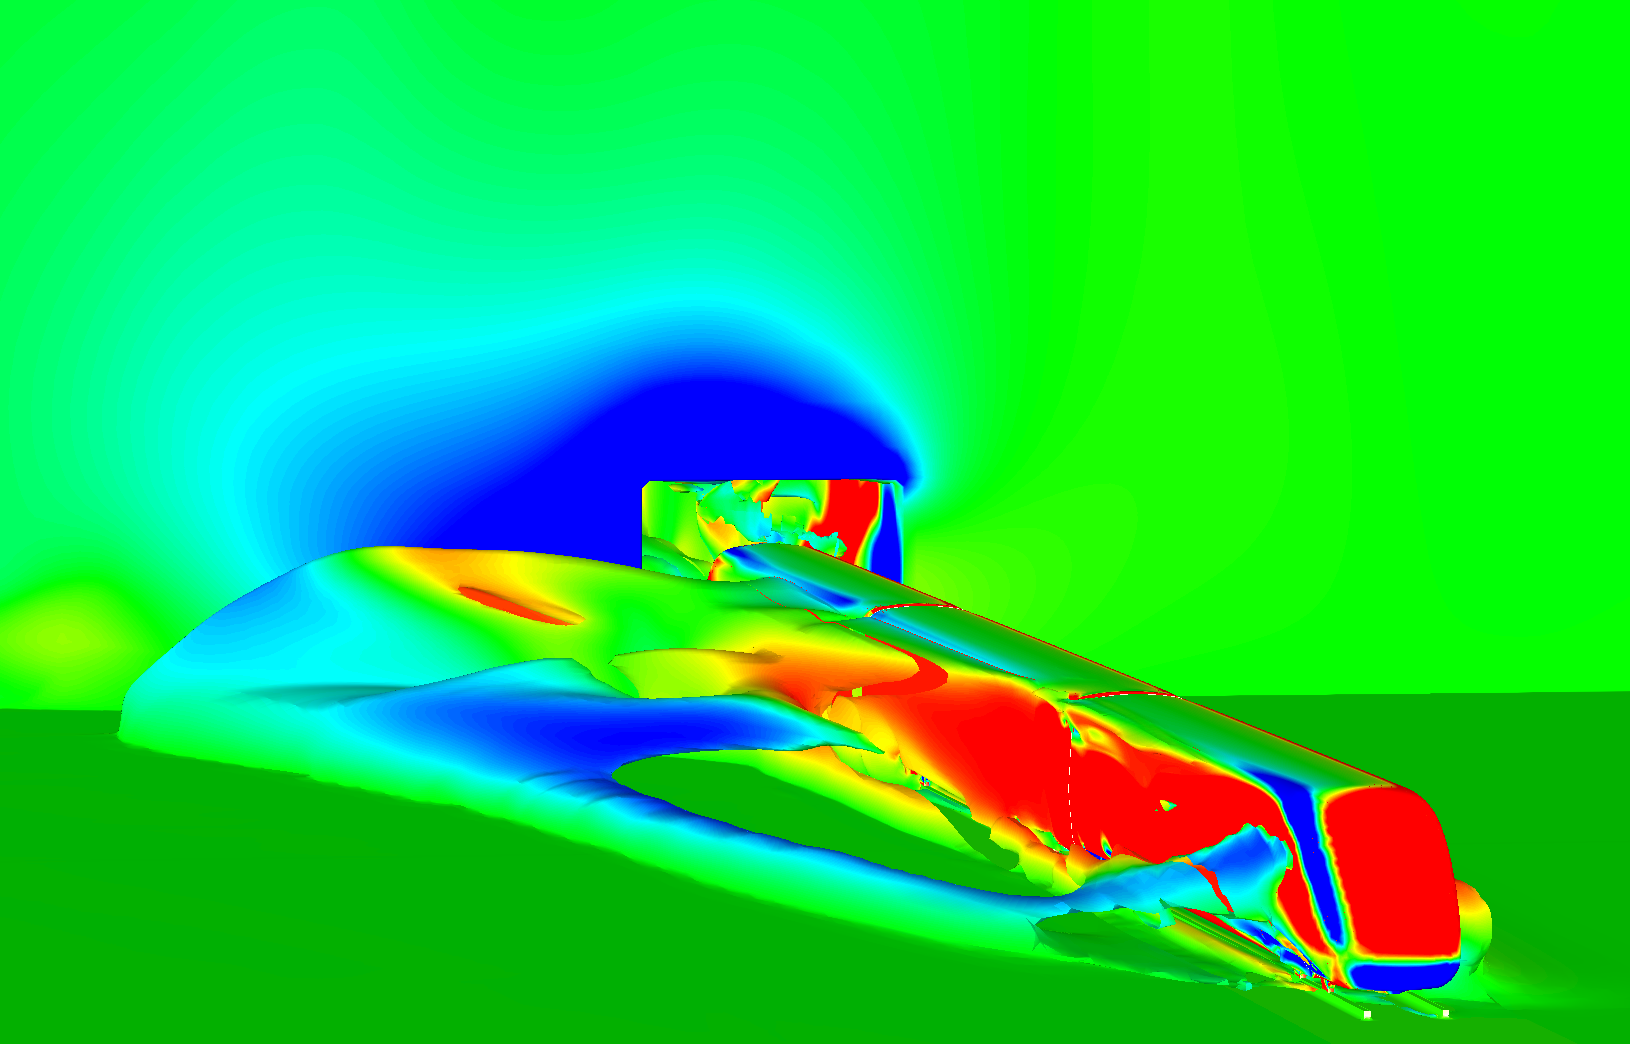
\includegraphics[width=\textwidth,height=0.4\paperheight,keepaspectratio]{figures/COVER_93_iso.png}}
\covercaption{Some explanation}

\firstabstract{\blindtext}
%\secondabstract{language}{\blindtext}
\keywords{Some stuff, More stuff, Stuff}

%\preface{\blindtext}
%\acknowledgement{\textit{Thanks to someone.}}
%\summary{\blindtext}

\paperwork{\blindtext}

\bibliography{mybib}


\begin{document}

\maketitle

%\phantomsection\addcontentsline{toc}{section}{Sammanfattning}
%\selectlanguage{swedish}
%\begin{abstract}Blabla swedish abstract\end{abstract}
% or a blank box
\part{Introduction}
% Real contents of report starts here
% Splitting it up to several files help when working together.
% Floatbarriers prevent figures from beeing placed into the next chapter.
\section{Introduction}
% \subsection{Background}
Due to the magnitude of the velocity of a high speed train (HST) the flow around it becomes an increasingly important factor. 
The unsteadiness and the different forces and moments that start acting on the train have a big impact on the stability of the train 
and safety and comfort of the passengers. This can probably be countered using damping in the bogies and coupling between the trains.
This is the reason behind this project. To find the forces and moments affecting the train 
and if it's the effects on discomfort and instability can be reduced.
In previous studies of HST instabilities it has either been purely aerodynamic or dynamic with simplified aerodynamic forces.
In this case it is intended to combine them to get an as accurate simulation as possible. 

\subsection{Purpose}
The purpose of this project is to combine two different fields, 
aerodynamics and dynamics, to accurately simulate the HST by
considering all the forces acting on the train in order to get an accurate model.
The goal of this project is to combine the aerodynamic forces that acts on a HST 
with the dynamics on the trains bogie and coupling. 
An interesting final result would be to find how sensitive the dynamics in the train is to varying velocity.

From vehicle dynamics side the focus of the project will be two folds:
\begin{itemize}
\item Create low-order mathematical and computational models for vibration dynamics and stability analysis of HST taking into account 
aerodynamic excitations. 
The models must implement the conventional bogie and conventional car-body coupling functional component mechanical models.
\item Using created models simulate the vibration dynamics and study stability of motion of HST for the two scenarios.
\end{itemize}

\subsection{Limitations}
Two different scenarios were studied. One where two trains meet each other and one where a single train has left a tunnel and is met by a strong wind gust. The model of the train used for the CFD simulations was an ICE2 train. The train consists of two locomotives and one car in the middle making it symmetrical. It has bogies and inter-car gaps. The parameters for the dynamics model were that of a typical HST. For the meeting trains the simulation was carried out at three different velocities, 67 m/s, 70 m/s and 73 m/s, which correspond to 240, 250 and 260 km/h respectively. For the scenario where the train coming out of a tunnel the speed of the train was 70 m/s and the speed of the wind gust was 35 m/s.

\subsection{Approach}
The aerodynamics was simulated with AVL-Fire CFD solver. For the double train, two train models were used with a moving mesh to simulate the two trains meeting each other. For the second scenario with the HST coming out of the tunnel a model of a ICE2 train in a simulated windtunnel with a moving crosswind was used. The forces and moments acting on the each train car on one of the trains were then handed over for the dynamics calculations.

The dynamics were simulated with a low order mathematical model using MATLAB and functional components for bogie and coupling.
The input were the forces and moments calculated from the CFD simulations and the forces acting on the wheels from the rail.
Unknown parameters, such as damping coefficients in the bogie, were decided by minimizing a cost function for comfort and stability.
As a last step, active damping was added to the model.%\FloatBarrier
\nocite{*}

%
\subsection{Theory}
The contact forces are calculated from creep in the contact plane.
The creep is defined as 
\begin{align}
 \xi_x    &= \frac{V_{wheel,x}}{V_0}\\
 \xi_\eta &= \frac{V_{wheel,\eta}}{V_0}
\end{align}
where $x$ is in the longitudinal direction, $\eta$ is perpendicular $x$ and the normal at the contact point and $V_0$ is the forward velocity of the train.

%Is it the purpose of these derivitions to not assume small deflections, as it is already solved as a nonlinear force.
\begin{figure}[htpb!]
 \centering
  \includegraphics[width=0.8\textwidth]{figures/QQ_0409.pdf}
 \caption{A plot!}
 \label{fig:plot} % Labels must come after caption!
\end{figure}

\begin{figure}[htpb!]
\centering
%\begin{tikzpicture}
%  \begin{axis}[xlabel=$x$,ylabel=$y$]
%   \addplot[color=blue,mark=*] plot coordinates { (0,2) (2,3) (3,1) };
%   \addlegendentry{Case 1}
%   \addplot[color=red,mark=x] plot coordinates { (0,0) (1,1) (2,1) (3,2) };
%   \addlegendentry{Case 2}
%  \end{axis}
% \end{tikzpicture}
 \caption{A tikz plot!}
 \label{fig:tikz_plot}
\end{figure}

Right side refers to the right in the forward direction of the train, i.e. the right wheel is not shown in figure \ref{fig:plot}.

The velocities can now be calculated as
% \begin{align}
% \omega_0 &= \frac{V_0}{r_0}\\
%  s       &= \begin{cases}+1&\text{if right side}\\-1&\text{if left side}\end{cases}\\
%  r       &= r[-s x_2]\\
%  w       &= s w_0 - x_2\\
%  \uv{d}  &= \begin{pmatrix}0\\w\\r\end{pmatrix}\\
%  \um{R}_z     &= \begin{pmatrix}
%         \cos[-\varphi_3] & -\sin[-\varphi_3] & 0\\
%         \sin[-\varphi_3] &  \cos[-\varphi_3] & 0\\
%         0                &  0                & 1
%      	\end{pmatrix} \\
%  \uv{V}_{wheel} &= \uv{\dot{x}} +\begin{pmatrix}V_0\\0\\0\end{pmatrix} + \um{R}_z \cdot (\uv{d} \times (\uv{\dot{\varphi}}+\begin{pmatrix}0\\\omega_0\\0\end{pmatrix}))
% \end{align}
where the $r$ is an interpolating function of the geometry of a standardized S1002 wheel profile \cite{railvehicledynamics_eandersson}.

\begin{table}[htpb!]
 \centering
 \caption{Explanation of variables for calculating the creep.}
 \begin{tabular}{c | l}
%  $\uv{x}$       & Translation vector of wheelset.\\
%  $\uv{\varphi}$ & Rotation vector of wheelset.\\
  $r_0$		 & Wheel radius at nominal contact point.\\
  $r$            & Wheel radius at current contact point.\\
  $w_0$		 & Lateral distance from COG to nominal contact point.\\
  $w$		 & Lateral distance from COG to current contact point.\\
  $V_0$		 & Nominal forward velocity of train.\\
  $\omega_0$	 & Nominal angular velocity of wheels.\\
  $\delta$	 & Inclination of wheels (positive).\\
  $s$		 & Side dependence, +1 for right side, -1 for left side.
 \end{tabular}
\end{table}

\subsubsection{Contact Patch Dimensions}
To calculate the forces the dimensions of the contact patch are required.
According to Hertz theory the dimensions are calculated as \cite{hallfasthetslara_bsundstrom} and \cite{railvehicledynamics_eandersson}
\begin{align}
 A+B    =& \frac12 \left(\frac{1}{r_{\eta,r}}+\frac{1}{r_{\eta,w}}+\frac{1}{r_{x,r}}+\frac{1}{r_{x,w}} \right)\\
 \nonumber B-A =& \frac12 \left(\left(\frac{1}{r_{x,r}}-\frac{1}{r_{\eta,r}}\right)^2 + 
                          \left(\frac{1}{r_{x,w}}-\frac{1}{r_{\eta,w}}\right)^2 +\right.\\
               &\left.   2\left(\frac{1}{r_{x,r}}-\frac{1}{r_{\eta,r}}\right)
                          \left(\frac{1}{r_{x,w}}-\frac{1}{r_{\eta,w}}\right)\cos[2\phi_z]\right)^\frac12\\
 \Psi   =& \sqrt[3]{\frac{3 N}{2 (A+B)} \left(\frac{1-\nu_w^2}{E_w} +\frac{1-\nu_r^2}{E_r}\right)}\\ 
 \theta =& \arccos\left[\frac{B-A}{A+B}\right]\\
 a      =& m \Psi\\
 b      =& n \Psi
\end{align}
where $m = m[\theta]$ and $n = n[\theta]$. There is no explicit expression for $m[\theta]$ or $n[\theta]$ but they can be solved numerically with (4.25) through (4.32) in \cite{contact_mechanics_kljohnson}. This has been done in table 8-1 in \cite{railvehicledynamics_eandersson} which values are used.

\begin{table}[htpb!]
 \centering
 \caption{Explanation of variables for calculating the creep.}
 \begin{tabular}{c | l}
  $N$                                     & Normal force in contact.\\
  $E_w,E_r$                               & Modulus of elasticity in the wheel and rail.\\
  $\nu_w,\nu_r$                           & Poissons ratio for the wheel and rail.\\
  $a,b$                                   & Contact patch dimension along $x$ and $\eta$.\\
  $r_{x,w},r_{x,r},r_{\eta,w},r_{\eta,r}$ & Radius around the respective axis for wheel and rail.\\
  $\phi_z$                                & The angle of the wheel.
 \end{tabular}
\end{table}
The radius $r_{\eta,r}$ is zero since the rail is straight. 
The other radii varies with the contact point and wheel profile. However they are approximated as constant for the contact geometry at a point far from the flange where the wheel is almost flat. In that case $r_{x,w}=\infty$ and $r_{\eta,w} = r$.
For the wheel the radius over the top of the rail is almost constant and be approximated as $r_{x,r} = 300$mm.
In this case $\eta$-axis is parallell with the $y$-axis.
The effect from the rotation of the wheel is also neglected, as this angle will always be small, i.e. linearisation of $cos[2\phi_z] \approx 1$. This simplifies the equations and with the approximations of the radii the variables $m$ and $n$ are constant.

The rest of the material parameters were set to $E_w = E_r = 200$ GPa and $\nu_w = \nu_r = 0.3$.

\end{document}
\subsubsection{Wheel Forces from Creep}
The creep forces are calculated with Kalker's linear theory \cite{railvehicledynamics_eandersson}.
The coefficients for the creep, $\uv{C} = \uv{C}[\frac{a}{b}]$, are interpolated from a set of data taken from table 8-2 in \cite{railvehicledynamics_eandersson}.

\begin{align}
 \uv{F}_{lin} &= - G a b \begin{pmatrix}
                          C_{11} \xi_x\\C_{22} \xi_\eta
                         \end{pmatrix}\\
 u            &= \frac{|\uv{F}_{lin}|}{\mu N}\\
 \uv{\hat{F}} &= \uv{F}_{lin} \begin{cases}
                  1-\frac{u}{3}+\frac{u^2}{27} &\text{if $u < 3$} \\
                  \frac{\mu N }{|\uv{F}_{lin}|} & \text{otherwise}
                 \end{cases}
\end{align}

The behaviour of the flange will be greatly simplified as done in \cite{appwheelrailcurvedtracks_jpombo}
\begin{align}
 F_{flange} = \begin{cases}
               k_{flange}( n_{flange}-x_2) & \text{if } x_2 >  n_{flange} \wedge s > 0 \text{ (right side)}\\
               k_{flange}(-n_{flange}-x_2) & \text{if } x_2 < -n_{flange} \wedge s < 0 \text{ (left side)}\\
               0                           & \text{otherwise}
              \end{cases}
\end{align}
where $F_{flange}$ acts in the $y$-axis and is added to  $F_y$.

The force vector $\uv{\hat{F}}$ is here acting on the contact plane, so to get the horizontal component
\begin{align}
 \uv{F} = \begin{pmatrix}
           F_x\\
           F_y
          \end{pmatrix} =
          \begin{pmatrix}
           \hat{F}_1\\
           \hat{F}_2\frac{\delta}{\sqrt{1+\delta^2}}+F_{flange}
          \end{pmatrix}
\end{align}

The contributions to the nonlinear force on the system will be
\begin{align}
 \uv{R}_e = \begin{pmatrix}
      F_x\\F_y\\0\\ 0\\r F_x\\-w F_x -w F_y \sin[\phi_3]
     \end{pmatrix}
\end{align}
which is assembled into $\uv{R}$ for each wheel.

%\subfile{Theory}\FloatBarrier
%\subfile{Method}\FloatBarrier
%\subfile{Results}\FloatBarrier
%\subfile{Conclusions}
%\subfile{Recommendations}

\printbibliography

\part{Appended Papers}

\paper{A stude of multiple crack interaction at rolling contact fatigue of rails}{\blindtext}

\paper{Assessment of acceleration modeling for fluid-filled porous media subjected to dynamic loading}{\blindtext}

\end{document}

